\chapter{Практичні результати}

У четвертому розділі представлено практичні результати
застосування алгоритму дифузії з сегментацією
та без із зазначенням вхідних даних.

\section{Практичні результати}

Вихідні зображення для побудови карти глибин
за допомогою описаних алгоритмів були взяті з набору стереопар,
зроблених в Мідлберійському коледжі в 2001~\cite{middlebury:ds:2001},
2003~\cite{middlebury:ds:2003}
та 2006~\cite{middlebury:ds:2006:1}~\cite{middlebury:ds:2006:2} роках.
На рисунку \ref{fig:stereopair:left} наведені ліві зображення зі стереопар,
для яких будувались карти глибин в даному розділі дисертації.
На рисунку \ref{fig:stereopair:right}
наведені праві зображення з тих же стереопар.

\begin{figure}[h]
\centering
    \begin{subfigure}[t]{0.32\textwidth}
        \centering
        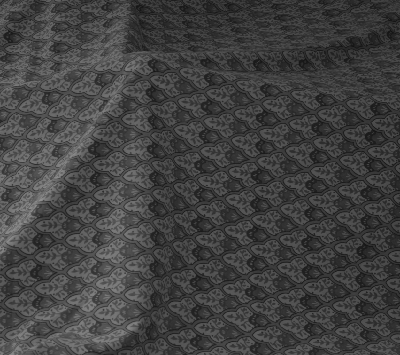
\includegraphics[width=\textwidth]{images/cloth_left}
        \caption{Тканина (Cloth1), $400 \times 355$ пікселів}
        \label{fig:cloth:left}
    \end{subfigure}
    \hfill
    \begin{subfigure}[t]{0.32\textwidth}
        \centering
        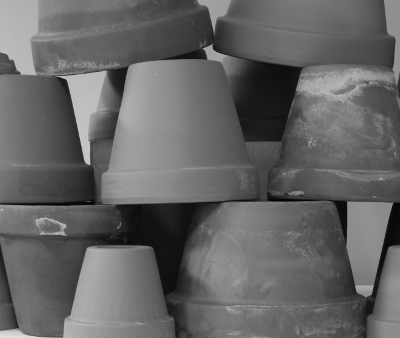
\includegraphics[width=\textwidth]{images/pots_left}
        \caption{Квіткові горщики (Flowerpots), $400 \times 338$ пікселів}
        \label{fig:flowerpots:left}
    \end{subfigure}
    \hfill
    \begin{subfigure}[t]{0.32\textwidth}
        \centering
        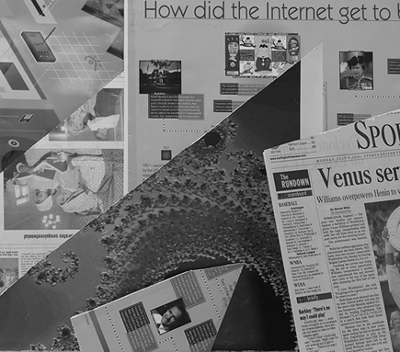
\includegraphics[width=\textwidth]{images/poster_left}
        \caption{Плакат (Poster), $400 \times 352$ пікселяв}
        \label{fig:poster:left}
    \end{subfigure}
    \caption{Ліві зображення стереопар}
    \label{fig:stereopair:left}
\end{figure}

\begin{figure}[h]
\centering
    \begin{subfigure}[t]{0.32\textwidth}
        \centering
        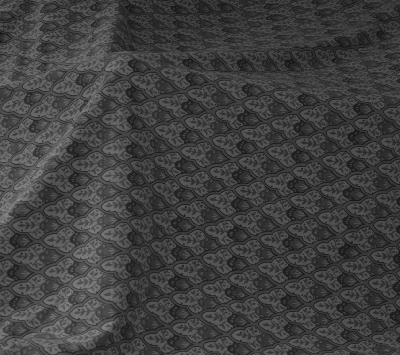
\includegraphics[width=\textwidth]{images/cloth_right}
        \caption{Тканина (Cloth1), $400 \times 355$ пікселів}
        \label{fig:cloth:right}
    \end{subfigure}
    \hfill
    \begin{subfigure}[t]{0.32\textwidth}
        \centering
        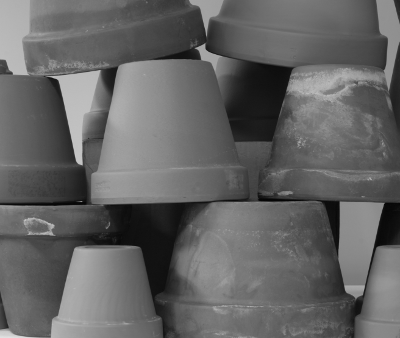
\includegraphics[width=\textwidth]{images/pots_right}
        \caption{Квіткові горщики (Flowerpots), $400 \times 338$ пікселів}
        \label{fig:flowerpots:right}
    \end{subfigure}
    \hfill
    \begin{subfigure}[t]{0.32\textwidth}
        \centering
        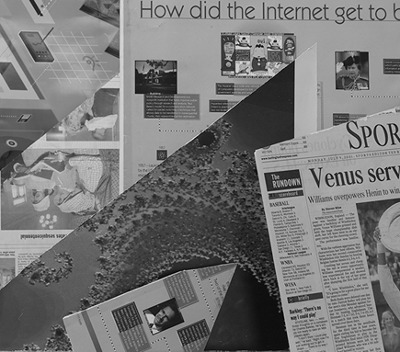
\includegraphics[width=\textwidth]{images/poster_right}
        \caption{Плакат (Poster), $400 \times 352$ пікселяв}
        \label{fig:poster:right}
    \end{subfigure}
    \caption{Праві зображення стереопар}
    \label{fig:stereopair:right}
\end{figure}

\section*{Висновки до розділу 4}
\addcontentsline{toc}{section}{Висновки до розділу 4}
